\section{Data Management and Access}
\label{sec:data}

This section presents how \hotpot\ manages user data in \dsnvm. 
We postpone the discussion of data durability and reliability to Section~\ref{sec:xact}.

\subsection{\nvm\ Page Morphable States}
One of \hotpot's design philosophies is to use one layer for both memory and storage 
and to integrate distributed memory caching and data replication.
To achieve this goal, we propose to impose {\em morphable} states on \nvm\ pages,
where the same \nvm\ page in \hotpot\ can be used both as a local memory cached copy to improve performance
and as a redundant data page to improve data reliability and availability.

We differentiate three states of a \nvm\ page:
active and dirty, active and clean, and inactive and clean,
and we call these three states {\em \dirty}, {\em \committed}, and {\em \redundant} respectively.
A page being clean means that it has not been updated since the last commit point;
committing a dirty page moves it to the clean state.
A page being active means that it is currently being accessed by an application,
while an \redundant\ page is a page which the application process has not mapped or accessed.
Several \hotpot\ tasks can change page states,
including page read, page write, data commit, data replication, page migration, and page eviction.
We will discuss how page states change throughout the rest of this section.
Figure~\ref{fig-data-eg} illustrates two operations that cause \hotpot\ data state changes.

\subsection{Data Organization}
\hotpot\ aims to support large-scale, data-intensive applications
on a fairly large number of nodes. %(\eg, at least a few racks)
Thus, it is important to minimize \hotpot's performance and scalability bottlenecks.
In order to enable flexible load balancing and resource management,
\hotpot\ splits the virtual address range of each dataset 
into {\em chunks} of a configurable size (\eg, 4\MB).
\nvm\ pages in a chunk do not need to be physically consecutive
and not all pages in a chunk need to exist on a node.

Each chunk in \hotpot\ is owned by an {\em owner node (\on)},
similar to the ``home'' node in home-based DSM systems~\cite{HLRC}.
%and to the primary node of distributed storage systems,
An \on\ maintains all the data and metadata of the chunk it owns.
%and serves requests from other nodes.
Other nodes, called {\em data node} or {\em \dn}, always fetch data from the \on\
when they initially access the data.
A single \hotpot\ node can simultaneously be the \on\ for some data chunks and the \dn\ for other chunks.
When the application creates a dataset, 
\hotpot\ \cd\ performs an initial assignment of \on{}s to chunks of the dataset.

Two properties separate \hotpot\ \on{}s from traditional home nodes.
First, %besides serving read data,
\hotpot\ \on\ is responsible for the reliability and crash consistency of the pages it owns,
besides serving read data and ensure the coherence of cached copies.
Second, \hotpot\ does not fix which node owns a chunk
and the location of \on\ adapts to application workload behavior dynamically.
Such flexibility is important for load balancing and application performance (see Section~\ref{sec:migration}).

\subsection{Data Reads and Writes}
\label{sec:readwrite}

\hotpot\ minimizes software overhead to improve application performance.
It is invoked only when a page fault occurs or when 
applications execute data persistence operations (see Section~\ref{sec:xact} for details of data persistence operations).

{
\begin{figure}[th]
\centering
\begin{center}
\centerline{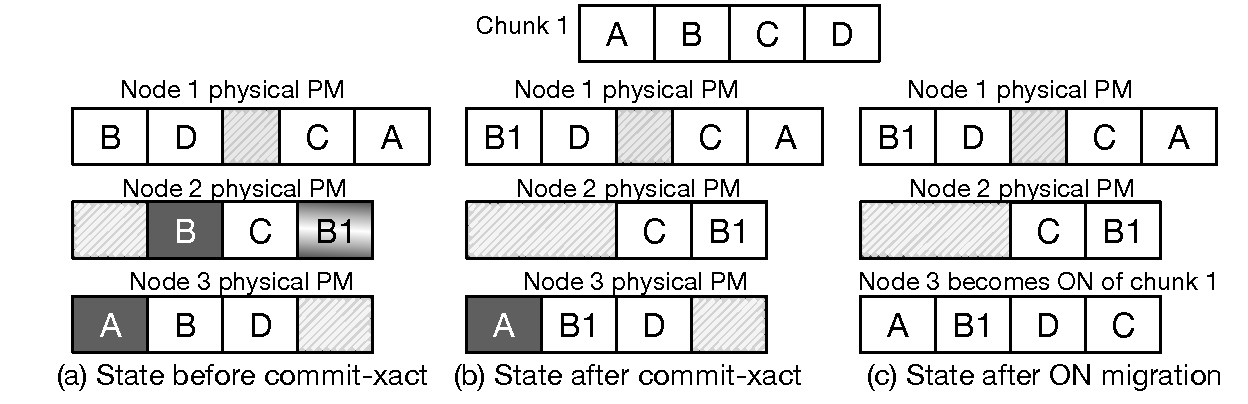
\includegraphics[width=\textwidth]{hotpot/Figures/data-eg.pdf}}
\end{center}
\caption[Data State Change Example.]
{Data State Change Example.
White, black, and striped blocks represent \committed, \redundant, and \dirty\ states.
Before commit, Node 2 and Node 3 both have cached copies of 
data page $B$. Node 2 has written to $B$ and created a \dirty\ page, $B1$.
During commit, Node 2 pushes the content $B1$ to its \on, Node 1.
Node 1 updates its \committed\ copy to $B1$ and also sends this update to Node 3.
Figure (c) shows the state after migrating the \on\ of chunk 1 from Node 1 to Node 3. 
After migration, Node 3 has all the pages of the chunk and all of them are in \committed\ states.
}
\label{fig-data-eg}
\end{figure}
}
When a page fault happens because of read, 
it means that there is no valid local page.
\hotpot\ first checks if there is any local \redundant\ page.
If so, it will move this page to the \committed\ state and establish a page table entry (PTE) for it.
Otherwise, there is no available local data and 
\hotpot\ will fetch it from the remote \on.
\hotpot\ writes the received data to a newly-allocated local physical \nvm\ page.
Afterwards, applications will use memory instructions to access this local page directly.


Writing to a \committed\ page also causes a page fault in \hotpot. 
This is because a \committed\ page can contribute towards user-specified degree of replication as one data replica,
and \hotpot\ needs to protect this committed version from being modified.
Thus, \hotpot\ write protects all \committed\ pages.
When these pages are written to (and generating a write page fault), 
\hotpot\ creates a local Copy-On-Write (COW) page
and marks the new page as dirty while leaving
the original page in \committed\ state.
\hotpot\ does not write protect this COW page, since it is already in the dirty state.

Following \hotpot's design philosophy to exploit hints from our targeted data-intensive applications,
we avoid propagating updates to cached copies at other nodes on each write and only do so at each application commit point.
Thus, all writes in \hotpot\ is local and only writing to a \committed\ page will generate a page fault.

Not updating remote cached copies on each write also has the benefit of reducing write amplification in \nvm.
In general, other software mechanisms and policies such as wear-aware \nvm\ allocation and reclamation 
and hardware techniques like Start-Gap~\cite{start-gap-micro09}
can further reduce \nvm\ wear.
We do not focus on \nvm\ wear in this paper and leave such optimizations for future work.

\subsection{\nvm\ Page Allocation and Eviction}
\label{sec:eviction}
Each \hotpot\ node manages its own physical \nvm\ space and performs \nvm\ page allocation and eviction.
Since physical pages do not need to be consecutive,
we use a simple and efficient allocation mechanism by maintaining a free page list
and allocating one page at a time.

\hotpot\ uses an approximate-LRU replacement algorithm that is similar to Linux's page replacement mechanism.
Different from Linux,
\hotpot\ distinguishes pages of different states.
\hotpot\ never evicts a \dirty\ page
and always tries to evict \redundant\ pages before evicting \committed\ pages.
We choose to first evict \redundant\ pages, 
because these are the pages that have not been accessed by applications
and less likely to be accessed in the future than \committed\ pages. %if a node accesses an \redundant\ page, it will become an \committed\ page.

Since both \redundant\ and \committed\ pages can serve as a redundant copy
for data reliability, \hotpot\ cannot simply throw them away during eviction.
The evicting node of a page will contact its \on{}, 
which will check the current degree of replication of the candidate pages 
and prioritize the eviction of pages that already have enough replicas. 
For pages that will drop below the user-defined replication degree after the eviction, 
the \on\ will make a new \redundant\ page at another node. %, if the eviction violates user-specified reliability requirements.

\subsection{Chunk \on\ Migration}
\label{sec:migration}
An \on{} serves both page read and data commit requests that belong to the chunks it owns.
Thus, the location of \on\ is important to \hotpot's performance.
Ideally, the node that performs the most reads and commits of data in a chunk 
should be its \on\ to avoid network communication.

By default, \hotpot\ initially spreads out a dataset's chunks to all \hotpot\ nodes in a round robin fashion
(other static placement policies can easily replace round robin).
Static placement alone cannot achieve optimal run-time performance.
\hotpot\ remedies this limitation by performing online chunk migration,
where one \on\ and one \dn\ of a chunk can switch their identities
and become the new \dn\ and new \on\ of the chunk.

\hotpot\ utilizes application behavior in recent history 
to decide how to migrate \on{}s.
Each \on\ records the number of page read requests
and the amount of committing data it receives in the most recent time window.

\on{}s make their migration decisions with a simple greedy algorithm based on the combination of two criteria:
maximizing the {\em benefit} while not exceeding a configurable {\em cost} of migration.
The benefit is the potential reduction in network traffic during remote data reads and commits.
The node that performs most data communication to the \on\ in recent history
is likely to benefit the most from being the new \on,
since after migration these operations will become local.
We model the cost of migration by the amount of data needed to copy to a node so that it has all the chunk data to become \on.

Once \hotpot\ has made a decision, it performs the actual chunk migration using 
a similar method as process and VM migration~\cite{OsmanEtAl02-Zap,Douglis87-Migration,Clark05-XenMigrate}
by temporary stopping commits to the chunk under migration
and resume them at the new \on\ after migration.

\if 0
    Once decided, a new ON node will be chosen. And the old ON will start to migrate pages to the
    the ON. During migration, the old ON is still the only valid ON in system. And, the old ON
    will keep serving page-fetch, but xact will be rejected.

    Once all pages are migrated from old ON to new ON, the old ON will 1) Tell CD that this region
    is migrated, hence CD can change its metadata. 2) Broadcast to nodes that currently have this
    region, that this region is migrated to new ON.
\fi

\if 0
\subsubsection{Replica Selection}
Apart from \on\ locations, the locations of data replicas can also affect application performance.
When a node has an \redundant\ page it can directly access it and avoid a remote page read. 
Thus, placing a data replica at a node that is likely to access the data in the future
can potentially improve performance.

\hotpot\ \on\ decides where to place an \redundant\ page during transaction commit with two criteria. 
%Currently, we use two criteria in selecting the location of a replica.
%replication gives us a chance to re-balance workloads
%happened in two occasions:
%when committing a transaction 
%and when evicting a \redundant\ page.
First, we use spatial locality to estimate the likelihood a node is going to access an \redundant\ page 
by the number of pages this node has read in the chunk that contains the \redundant\ page.
The second consideration is to prevent thrashing.
When a node runs out of space, it will first evict \redundant\ pages (Section~\ref{sec:eviction})
and assigning \redundant\ pages to such nodes will cause thrashing.
Thus, \hotpot\ compares the total \nvm\ free space of a node and avoids assigning 
\redundant\ pages to nodes with space pressure.
\fi
